\chapter{Математические модели поглощения гелия микросферами и сорбентом на их основе в статических условиях}
 \label{section_2}
 
\section{Модель типа <<растворение-диффузия>> для изучения проникновения гелия внутрь микросфер}
 \label{section_2_1}
 
Избирательная проницаемость гелия через стенку микросферы происходит в следствие малости кинетического диаметра молекулы гелия и соответствует разделу газоразделения с помощью непористых мембран \cite{Mulder}. Это явление можно разделить на три этапа: 1) растворение гелия в приповерхностном слое материала стенки микросферы; 2) диффузия гелия сквозь стенку микросферы; 3) десорбция гелия в полость частицы. В равновесном приближении объем гелия, растворившегося вблизи поверхности микросферы, зависит от давления в свободном объёме и определяется законом Генри. 

Транспорт гелия через стенку микросферы описывается уравнением диффузии в сферическом приближении:
\begin{equation}
\label{eq:FikHenry_hellium_permeation_model}
\pd{c}{t}=\frac{D}{r^2}\pd{}{r}\left( r^2 \pd{c}{r} \right),
\end{equation}
где $c(t,r)$ -- концентрация гелия в стенке микросферы в зависимости от времени и расстояния до центра частицы ($t > 0$, $a \leq r \leq b$); $D$ -- коэффициент диффузии гелия в материале стенки микросферы; $a$, $b$ -- радиусы полости и внешний радиус микросферы соответственно. 

Рассматривая задачу диффузии в квазистационарном приближении (когда профиль концентрации устанавливается быстро при заданных на границах концентрациях газа), пренебрегают производной по времени 
\begin{equation}
\label{eq:FikHenry_hellium_permeation_model_quasistat}
c = c(r)
\end{equation}
и к уравнению (\ref{eq:FikHenry_hellium_permeation_model}) добавляют следующие граничные условия:
\begin{equation}
\label{eq:FikHenry_hellium_permeation_model_conditions}
c(t, a)  = k_S p_2,\quad
c(t, b)  = k_S p_1,\quad
\end{equation}
где $p_1$, $p_2$ -- давления гелия снаружи и внутри микросферы соответственно; $k_S$~--~коэффициент растворимости гелия в материале стенки микросферы в соответствии с законом Генри.

Решением (\ref{eq:FikHenry_hellium_permeation_model}) с учётом (\ref{eq:FikHenry_hellium_permeation_model_quasistat}) и (\ref{eq:FikHenry_hellium_permeation_model_conditions}) является выражение, описывающее профиль концентрации:
\begin{equation}
\label{eq:eq:FikHenry_hellium_permeation_model_solution}
c(r) = -\frac{k_S(p_1-p_2)ab}{(b-a)r}+\frac{k_S(bp_1-ap_2)}{b-a}\quad
(a \leq r \leq b).
\end{equation}

Массовый поток гелия через любое сечение $r=r_0$ ($a\leq r_0 \leq b$) с площадью $S_0=4\pi r_0^2$ равен
\begin{equation}
\label{eq:FikHenry_hellium_permeation_model_massflow}
q = -D \left. \pd{c}{r} \right|_{r=r_0}S_0=-\frac{C_m S \gamma}{d}(p_1-p_2),
\end{equation}
где $C_m = D k_s$ -- коэффициент проницаемости материала стенки; $S=4 \pi b^2$~--~площадь поверхности микросферы; $\gamma$ = $a/b$; $d=b-a$ -- толщина стенки микросферы.

Массовый поток для сферической мембраны (\ref{eq:FikHenry_hellium_permeation_model_massflow}) отличается от потока для плоской мембраны \cite{Hvang, Ditnerskiy, Mulder} множителем $\gamma$. В случае, когда стенки микросфер очень тонкие $a \approx b$ им можно пренебречь.

\section{Математическая модель поглощения гелия в предположении одинаковости физических и геометрических свойств микросфер}
 \label{section_2_2}

Объем гелия, растворённого в материале стенки микросферы, зависит от коэффициента растворимости Освальда $S_{\mathrm{Os}}$ равного отношению объёма растворённого газа к единице массы вещества при атмосферном давлении, равном $1,0 \cdot 10^5$~Па. Для гелия и бездефектного кристалла кварца $S_{\mathrm{Os}}=(5,9 \div 11,8) \cdot 10^{-13}$~см$^3$/(г$\cdot$Па) \cite{Argunova_Sorokin}. В экспериментах, проводимых в реакторе, объем которого составляет около $3\cdot 10^{-2}$~м$^3$, при максимальных давлениях порядка $6,1\cdot 10^5$~Па, объёмом гелия, растворённого в материале стенки микросферы, можно пренебречь.

Используя полученную формулу массового потока гелия в частицу  (\ref{eq:FikHenry_hellium_permeation_model_massflow}), задача поглощения одной микросферой гелия, находящегося в реакторе с внешним парциальным давлением $p_1$ и внутренним $p_2$ сводится к дифференциальног решению уравнения:
\begin{equation}
\label{eq:one_particle_permiation}
\dt{M^0_2}= \frac{C_m\gamma S}{d}(p_1-p_2),
\end{equation}
где $M^0_2(t)$ -- масса гелия внутри одной микросферы, как функция от времени $t$. 

Рассмотрим процесс поглощения/выделения гелия из частицы на примере сосуда с одинаковыми микросферами, заполненного газом (гелием) равномерно по всему объёму. В начальный момент времени микросферы одинаково заполнены.  Считая, что они распределены равномерно по всему объёму и, что процесс поглощения происходит одинаково во всех точках системы, замкнутая система уравнений, описывающая этот процесс, имеет вид:
\begin{equation}
\left\{
\begin{array}{l}
\label{eq:permeation_even_laws}
\displaystyle\dt{M_2(t)}= k\frac{C_m\gamma S}{d}(p_1(t)-p_2(t)), \\
%\label{eq:permeation_even_laws_M1}
M_1(t)+M_2(t)=M_0
\end{array}
\right.
\end{equation}
с замыкающими соотношениями
\begin{equation}
\label{eq:permeation_even_laws_relations}
\displaystyle p_1(t) = \frac{M_1(t)R_{He}T}{V_1},\quad p_2(t)=\frac{M_2(t)R_{He}T}{V_2},
\end{equation}
где  $M_1(t)$, $M_2(t)$ -- масса гелия, находящаяся в свободном объеме и полостях всех микросфер, во время $t$; $M_0$ -- суммарная масса гелия в системе; $k$ -- количество микросфер в системе; $R_{He}$ -- универсальная газовая постоянная для гелия; $T$ -- температура газа; $V_1$ -- свободный объем реактора; $V_2$ -- объем  полостей всех микросфер; $S$ -- площадь поверхности одной микросферы; $d$ -- толщина стенки микросферы; $C_m$ -- коэффициент проницаемости материала стенки микросферы. 

Первое соотношение (\ref{eq:permeation_even_laws}) описывает закон поглощения/выделения гелия всеми микросферами системы, второе -- закон сохранения массы в системе. 

Используя  (\ref{eq:permeation_even_laws_relations}) и соотношения, вытекающие из геометрии для микросфер с радиусом полости $r$ и внешним радиусом $R$,
\[
S=4\pi R^2,\quad d=R-r,\quad V_2=k\frac{4}{3}\pi r^3,
\]
в терминах переменных $p_1(t)$ и $p_2(t)$ система уравнений (\ref{eq:permeation_even_laws}) записывается в виде:
\begin{equation}
\label{eq:permeation_even_laws_p} 
\left\{
\begin{array}{l}
\displaystyle \dt{p_2}  =  K(p_1-p_2), \\
p_1+\alpha p_2  =  p_1^0 + \alpha p_2^0, 
\end{array}
\right.
\end{equation}
при начальных условиях
\begin{equation}
\label{eq:permeation_even_laws_cauchy} p_1|_{t=0}=p_1^0,\quad p_2|_{t=0}=p_2^0,
\end{equation}
здесь $\alpha=V_2/V_1$; $K = C_m R_{He} T\displaystyle\frac{3}{\gamma rd}$, а $p_1^0$, $p_2^0$ -- начальные парциальные давления гелия в свободном объёме и внутри полостей. 

Решением (\ref{eq:permeation_even_laws_p}) и (\ref{eq:permeation_even_laws_cauchy}) будут следующие функции:
\begin{eqnarray}
\label{eq:permeation_even_p1}
p_1(t) & = & \frac{p_1^0 + \alpha p_2^0}{1+\alpha} - \frac{\alpha}{1+\alpha}(p_2^0-p_1^0)e^{-K(1+\alpha)t}, \\
\label{eq:permeation_even_p2}
p_2(t) & = & \frac{p_1^0 + \alpha p_2^0}{1+\alpha} + \frac{1}{1+\alpha}(p_2^0-p_1^0)e^{-K(1+\alpha)t}.
\end{eqnarray}

Из вида функций $p_1(t)$ и $p_2(t)$ легко понять, что они, начиная со своих начальных значений при $t=0$, экспоненциально стремятся к равновесному давлению 
\begin{equation}
\label{eq:permeation_even_pinfty}
p_\infty=\displaystyle\frac{p_1^0 + \alpha p_2^0}{1+\alpha},
\end{equation}
а скорость стремления к асимптоте зависит от величины $K(1+\alpha)$. Схематично решения в зависимости от различных значений $p_1^0$ и $p_2^0$ изображены на рисунке~\ref{pic:permeation_even}. Случай $p_1^0=p_2^0$ приводит к постоянному решению уравнения (\ref{eq:permeation_even_laws_p}) 
\[
p_1(t)=p_2(t)=p_1^0=p_2^0=p_\infty\quad (t>0).
\]


\begin{figure}[ht] 
	\begin{minipage}[ht]{0.49\linewidth}\centering
			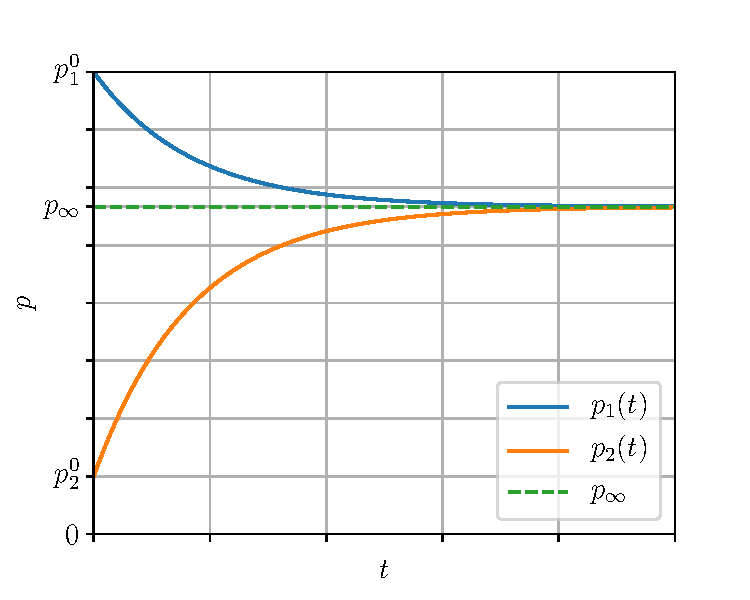
\includegraphics[width=\textwidth]{part_2/sorb_even} \\ а)
	\end{minipage}
	\hfill
	\begin{minipage}[ht]{0.49\linewidth}\centering
		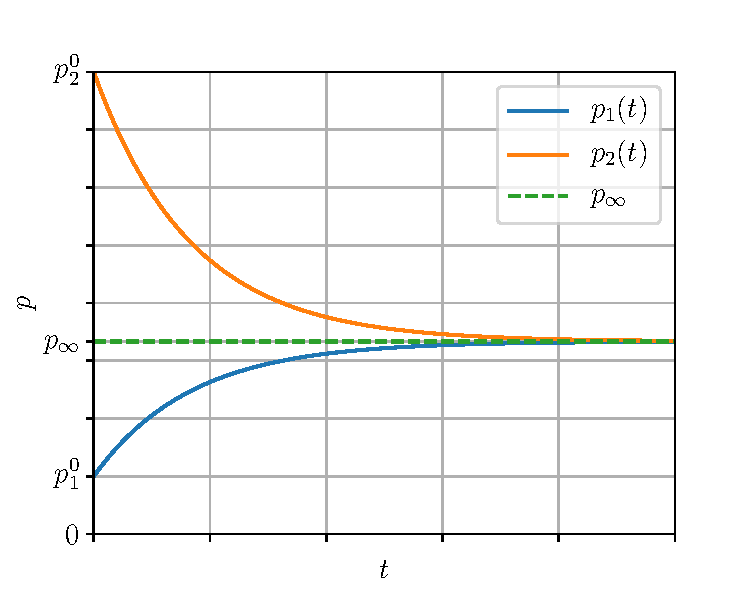
\includegraphics[width=\textwidth]{part_2/desorb_even} \\ б)
	\end{minipage}

	\caption{Схематичное изображение решения задачи о поглощении гелия одинаковыми микросферами: a) задача сорбции гелия микросферами ($p_1^0>p_2^0$); б) задача десорбции гелия микросферами ($p_1^0<p_2^0$).}
	\label{pic:permeation_even}
\end{figure}


\todo{Сравнение с экспериментом}


\section{Математическая модель поглощения гелия в предположении дисперсионного распределения микросфер по геометрическим и физическим параметрам}
\label{section_2_3}

\subsection{Основные уравнения}
\label{section_2_3_1}

Не всегда имеется возможность экспериментально получить однородные по размерам и коэффициентам проницаемости частицы сорбента  (например, при травлении поверхности ценосфер \cite{ICCT_cenosphere_permeation} или при создании композитного сорбента \cite{Vereshchagin:2016_Vapour_Helium}). Целью данного параграфа является построение математической модели сорбции гелия микросферами с учётом их дисперсионного распределения по геометрическим и физическим параметрам в рамках задачи поглощения гелия в замкнутом объёме и предположений, обозначенных в разделе \ref{section_2_1}.

В соответствии с (\ref{eq:FikHenry_hellium_permeation_model_massflow}) постулируем, что поток массы в $i$-ю микросферу ($i=\overline{1,n}$) определяется соотношением
\begin{equation}
\label{eq:uneven_p1_permeation_law}	
j^{(i)}(t) = C_m^{(i)}(p_1(t)-p_{21}^{(i)}(t)),
\end{equation}
где $C_m^{(i)}$	-- коэффициент проницаемости $i$-й микросферы, включающий весь комплекс характеристик описывающих конкретную частицу;
$p_{21}^{(i)}(t)$ -- давление гелия в полости $i$-й микросферы;
$p_1(t)$ -- давление гелия в сосуде. В данном случае коэффициент проницаемости $C_m^{(i)}$ является интегральной характеристикой $i$-й частицы и зависит от ее формы, толщины, температуры, поглощаемого газа и т.д.

С учетом (\ref{eq:uneven_p1_permeation_law}) и  сказанного выше  математическая модель поглощения гелия микросферами записывается следующим образом:	
\begin{equation}
\label{eq:M21i_relations}
\dt{M_{21}^{(i)}(t)}  =  C_m^{(i)}(p_1(t)-p_{21}^{(i)}(t)) \quad (i=1,...,n);
\end{equation}
\begin{equation}
\label{eq:uneven_conserv_law}
\sum\limits_{i=1}^n M_{21}^{(i)}(t)+M_1(t)   =   M_0.
\end{equation}
Здесь $M_{21}^{(i)}(t)$ -- масса гелия в $i$-й микросфере в момент времени $t$; $M_1(t)$ -- масса гелия в свободном объеме системы в момент времени $t$; $M_0$ -- суммарная масса гелия в системе.

Замыкающие соотношения (для идеального газа) имеют вид
\begin{equation}
\label{eq:uneven_closing_relations}
p_{21}^{(i)}(t) =\frac{M_{21}^{(i)}(t)}{V_{21}^{(i)}} R_1 T, \quad p_{1}(t) =\frac{M_{1}(t)}{V_{1}} R_1 T,
\end{equation}	
где $R_1$ -- универсальная газовая постоянная для гелия; $T$ -- температура в системе; $V_{21}^{(i)}$ -- объем полости $i$-й частицы; $V_1$ -- свободный объем системы.

Начальное состояние системы определяется условиями
\[
M_{21}^{(i)}|_{t=0} =0 \quad (i=1,...,n),\quad M_1|_{t=0} = M_0.
\]


С помощью выражений (\ref{eq:uneven_closing_relations}) уравнения (\ref{eq:M21i_relations}) (для всех $i=1,...,n$) разрешаются следующим образом:
\begin{equation}
\label{eq:M21i_def}
M_{21}^{(i)}(t)=\alpha_i\beta_i\int\limits_{0}^{t}M_1(\tau) \mathrm{e}^{\beta_i (\tau-t)} d\tau;
\end{equation}
\begin{equation}
\label{eq:uneven_alpha_beta_def}
\alpha_i = \frac{V_{21}^{(i)}}{V_1},\quad \beta_i = \frac{C_m^{(i)}}{V_{21}^{(i)}}R_1T.
\end{equation}
Подставляя (\ref{eq:M21i_def}) в (\ref{eq:uneven_conserv_law}), получаем следующую математическую модель процесса поглощения гелия микросферами:
\begin{equation}
\label{eq:uneven_descrete_model}
M_1(t)=M_0-\int\limits_{0}^{t}  M_1(\tau)  G(t-\tau) d\tau, \quad
G(x) = \sum\limits_{i=1}^{n}\alpha_i \beta_i  \mathrm{e}^{-\beta_i x}.
\end{equation}
%\begin{equation}
%\label{eq:uneven_M1_start_condition}
%M_1(0) = M_0.
%\end{equation}
Здесь $\alpha_i$ -- безразмерная характеристика внутреннего объема $i$-й микросферы; $\beta_i$ -- характеристика проницаемости $i$-й микросферы, с$^{-1}$.

%В общем виде уравнение (\ref{eq:uneven_descrete_model}) представляет собой уравнение Фредгольма второго рода с неизвестной функцией $M_1(t)$ и заданном ядром $G(x)$ при известных параметрах $\alpha_i$, $\beta_i$ и имеет решение. Однако, как правило, ставится обратная задача: по известной функции $M_1(t)$ определить такие параметры среды, как распределение коэффициентов проницаемости стенок микросфер, распределение внутренних объемов микросфер и др. Для получения решения обратной задачи необходимо упростить уравнения (\ref{eq:uneven_descrete_model}). 

\subsection{Основные свойства модели}

Уравнение (\ref{eq:uneven_descrete_model}) представляет собой уравнение Фредгольма второго рода с неизвестной функцией $M_1(t)$ и заданном ядром $G(x)$ при известных параметрах $\alpha_i$, $\beta_i$. Рассмотрим основные свойства этих уравнений применительно к задачи сорбции.


\textbf{Классы эквивалентных частиц.} Из выражения (\ref{eq:uneven_descrete_model}) для ядра $G(x)$  видно, что для микросфер, имеющих один и тот же коэффициент проницаемости $\beta_i=\beta_j$ для некоторых $i$, $j$, есть возможность привести подобные слагаемые, при этом происходит сложение внутренних объёмов $\alpha_i$ и $\alpha_j$. Таким образом, сокращается количество слагаемых функции $G(x)$.


Разделим все микросферы на классы частиц, эквивалентных по коэффициенту проницаемости:  $i$-я и $k$-я частицы принадлежат одному классу тогда и только тогда, когда для них справедливо $\beta_i=\beta_k$. Из уравнения (\ref{eq:M21i_def}) следует, что масса гелия, проникшего в микросферы $j$-о класса, определяется выражением
\begin{equation}
\label{eq:m21j_def}
\sum\limits_{i \in H_j} M_{21}^{(i)}(t) = \left(\sum _{i \in H_j} \alpha_i \right) \beta_{i(j)} \int\limits_{0}^{t}M_1(\tau) e^{\beta_{i(j)} (\tau-t)} d\tau,
\end{equation}
где $H_j$ -- множество индексов частиц, соответствующих $j$-му классу; $i(j)$ -- индекс любой частицы, принадлежащей $j$-му классу.

Результаты сравнения выражений (\ref{eq:M21i_def}) и (\ref{eq:m21j_def}) показывают, что каждому коэффициенту проницаемости $\beta$ можно поставить в соответствие суммарный внутренний объем всех частиц с таким значением $\beta$. В этом случае существует однозначная функция $\alpha=f(\beta)$ с указанными свойствами.

Не уменьшая общности, можно считать, что уравнение (\ref{eq:uneven_descrete_model}) записано для классов,  близких по характеристикам частиц, а параметры $\alpha_i$ соответствуют интегральным характеристикам этих классов. 

\textbf{Равновесное давление.}
Предположим, что в реакторе установилось равновесие, т.е. давление гелия в частицах $p_{21,\infty}^{(i)}$ стало равно давлению гелия вне частиц $p_{1,\infty}$. Используя уравнения состояния идеального газа, эти условия записываются следующим образом
\begin{equation}
\label{eq:uneven_equil_cond}
\frac{M_{21,\infty}^{(i)}}{V_{21}^{(i)}} R_1 T = \frac{M_{1\infty}}{V_1}R_1 T \quad (i=1 \ldots n),
\end{equation}
где $M_{1\infty}$ -- безразмерное значение равновесной массы гелия в реакторе вне частиц; $M_{21,\infty}^{(i)}$ -- безразмерное равновесное значение массы гелия в $i$-й частице.

С использованием равенств (\ref{eq:uneven_equil_cond}), масса гелия попавшего в частицы $M_{21,\infty}$ выражается по следующей формуле
\begin{equation}
\label{eq:uneven_M21_infty}
M_{21,\infty} = \sum\limits_{i=1}^{n}M_{21,\infty}^{(i)}=\alpha M_{1\infty}, 
\end{equation}
где $\alpha = \displaystyle\frac{\sum\limits_{i=1}^{n} V_{21}^{(i)}}{V_1}$ -- безразмерная характеристика системы, являющаяся отношением суммарного объема полостей частиц к свободному объему в реакторе, которую можно выразить через известные данные о распределении частиц по размерам, объем реактора, массу используемого сорбента и др.

Используя связь массы и давления (\ref{eq:uneven_closing_relations}) и закон сохранения массы в системе ($M_{1\infty}+M_{21,\infty}=M_0$) из уравнения (\ref{eq:uneven_M21_infty}) получается выражение 
\begin{equation}
\label{eq:uneven_M1_infty}
p_{1\infty} = \frac{p_0}{1+\alpha},
\end{equation}
где $p_0$ -- начальное давление в системе, соответствующее массе $M_0$, которое совпадает с аналогичным соотношением для монодисперсной модели (\ref{eq:permeation_even_pinfty}) при $p_1^0=p_0$, $p_2^0=0$.


\subsection{Различные виды записи модели и частные случаи}
\label{section_2_3_3}

%Рассмотрим различные упрощения:
%\begin{enumerate}
%	\item Монодисперсное распределение частиц. Полагаем $\alpha_i=\alpha_0$, $\beta_i=\beta_0$ $(i=1,...,n)$. В этом случае уравнения (\ref{eq:uneven_descrete_model}) преобразуются в модель (\ref{eq:permeation_even_laws}) со всеми вытекающими последствиями.
%	\item Распределение линейных размеров микросфер по нормальному закону при фиксированной толщине стенки.  В предположении, что проницаемость материала стенки микросферы одни и те же, выражение для коэффициента проницаемости можно представить в виде
%	\[
%	C_m^{(i)} = C_m S/d,
%	\]
%	где $S$ -- площадь микросферы, через которую происходит проникание; $d$~--~толщина стенки микросферы; $C_m$ -- коэффициент проницаемости материала стенки микросферы, который зависит от 
%	вещества и структуры стенки микросферы, температуры, исследуемого газа. В рассматриваемом случае будем полагать, что радиусы полости микросфер распределены по нормальному закону. Тогда
%	\[
%	C_m(r) =\frac{4 C_m \pi r^2}{d},\quad V_{21}(r)=(4/3) \pi r^3, \quad r \in N[r_0, \sigma],
%	\]
%	где $N[r_0, \sigma]$ -- нормальное распределение с математическим ожиданием $r_0$ и дисперсией $\sigma$. При данных предположениях упрощением модели (\ref{eq:uneven_descrete_model})  является модель, полученная в работе \cite{Ver_Norm_Dist}, в которой показано, что при моделировании процесса сорбции на микросферах с фиксированной толщиной стенки при параметрах микросфер близким к параметрам микросфер МСВ-1Л варьирование дисперсии $\sigma$ не оказывает существенного влияния, т.е. при описании достаточно использовать более простую модель с монодисперсным распределением (\ref{eq:uneven_descrete_model}).
%	\item Известно распределение частиц и толщин стенок микросфер по размеру. Остановимся подробнее на этом случае.
%\end{enumerate}

\textbf{Монодисперсное распределение частиц.}
Полагаем $\alpha_i=\alpha_0$, $\beta_i=\beta_0$ $(i=1,...,n)$. В этом случае уравнения (\ref{eq:uneven_descrete_model}) преобразуются в модель (\ref{eq:permeation_even_laws}) со всеми вытекающими последствиями.

\textbf{Переход от дискретной модели к непрерывной.}
Переходя от дискретной модели (\ref{eq:uneven_descrete_model}) к непрерывной, постулируем существование функции $p(\beta)$, такой что 
\begin{equation}
\label{eq:uneven_pbeta_def}
\alpha = \int_{\beta_1}^{\beta_2} p(\beta) d\beta\quad
(0 \leq \beta_1 \leq \beta_2).
\end{equation}
Здесь $\alpha$ -- суммарный безразмерный внутренний объём частиц с проницаемостями от $\beta_1$ до $\beta_2$. Тогда уравнение (\ref{eq:uneven_descrete_model}) принимает вид
\begin{equation}
\label{eq:uneven_cont_model}
\begin{array}{rl}
M_1(t)=M_0-\int\limits_{0}^{t}  M_1(\tau)  G(t-\tau) d\tau, & 
G(x) = \int\limits_{0}^{\infty}\beta p(\beta)  \mathrm{e}^{-\beta x} d\beta,\\
\end{array}
\end{equation}


\textbf{Учёт распределения частиц по размеру при постоянном коэффициенте проницаемости стенки микрсферы.}
Пусть заданы плотность распределение радиусов полостей микросфер в зависимости от радиуса полости $q(r)$ и коэффициент проницаемости материала стенки микросферы $C_m$, который для исследуемого типа поглотителя считается постоянным.

Из соотношения (\ref{eq:uneven_p1_permeation_law}) и (\ref{eq:FikHenry_hellium_permeation_model_massflow}) следует, что
\begin{equation*}
\label{eq:uneven_Cmi_V21i_def}
C_m^{(i)} = \frac{C_m S_i \gamma_i}{d_i}, \quad V_{21}^{(i)} = 4/3\pi r_i^3
\end{equation*}
($S_i=4 \pi (r_i+d_i)^2$ -- площадь поверхности $i$-й микросферы, через которую происходит транспорт газа; $d_i$ -- толщина стенки $i$-й микросферы). Тогда из (\ref{eq:uneven_alpha_beta_def}) получаем
\begin{equation}
\label{eq:uneven_beta_reduction}
\beta_i = \frac{3}{r_i d_i} \left(1+\displaystyle\frac{d_i}{r_i}\right)  C_m R_1 T, \quad (i=1,\ldots, k).
\end{equation}

Предположим также, что существуют взаимно однозначная функция и функция, обратная к ней:
\begin{equation*}
\label{eq:uneven_betar_con}
\beta = \beta(r), \quad r=r(\beta) \quad (r_1 \leq r \leq r_2, \beta_1 \leq \beta \leq \beta_2),
\end{equation*}
такие что 
\[
\frac{d\beta}{dr} < 0 \quad (r_1 \leq r \leq r_2),
\]
где $[r_1, r_2]$ -- исследуемый интервал радиусов полостей, а $[\beta_1, \beta_2]$ -- соответствующий ему интервал изменения параметра поглощения ($\beta_1=\beta(r_2)$, $\beta_2 = \beta(r_1)$).

В этом случае из уравнения (\ref{eq:uneven_pbeta_def})  следует
\begin{equation*}
V_1 \int\limits_{\beta_1}^{\beta}p(\beta)d\beta = k \int\limits_{r(\beta)}^{r_2}(4/3)\pi r^3 q(r) dr.
\end{equation*}
($q(r)$ -- плотность распределения радиуса полости микросфер; $k$ -- количество микросфер в системе). Из этого выражения получаем зависимость между плотностями распределения $p(r)$ и $q(r)$
\begin{equation}
\label{eq:uneven_pq_con}
p(r) = - \frac{4/3 \pi r^3 k}{V_1}  q(r) \left( \frac{d\beta}{dr} \right)^{-1}.
\end{equation}
С учетом (\ref{eq:uneven_pq_con}) уравнения (\ref{eq:uneven_cont_model}) принимают вид
\begin{equation}
\label{eq:uneven_cont_model_qr}
\begin{array}{c}
M_1(t)=M_0-\int\limits_{0}^{t}  M_1(\tau)  G(t-\tau) d\tau, \\
G(x) = \displaystyle\frac{4/3 \pi k}{V_1} \int\limits_{r_1}^{r_2}\beta(r) r^3  \mathrm{e}^{-\beta(r) x} q(r) dr.
\end{array}
\end{equation}

\textbf{Нормальное распределение радиусов частиц при фиксированной толщине стенки.}
Рассмотрим ситуацию распределения линейных размеров микросфер по нормальному закону при фиксированной толщине стенки.  В предположении, что проницаемость материала стенки микросферы одни и те же, выражение для коэффициента проницаемости (\ref{eq:uneven_beta_reduction})  можно представить в виде
\[
\beta(r) = \frac{3 C_m}{r d}\left(1+\displaystyle\frac{d}{r}\right) R_1 T, \quad r \in N[r_0, \sigma],
\]
где $N[r_0, \sigma]$ -- нормальное распределение с математическим ожиданием $r_0$ и дисперсией $\sigma$, задаваемое плотностью распределения 
\[
q(r) = \frac{1}{\sigma\sqrt{2\pi}}e^{-\displaystyle\frac{(r-r_0)^2}{2\sigma^2}}.
\]

При данных предположениях упрощением модели (\ref{eq:uneven_cont_model_qr})  является модель, рассмотренная в работе автора \cite{Ver_Norm_Dist}, в которой показано, что при моделировании процесса сорбции на микросферах с фиксированной толщиной стенки при параметрах микросфер близким к параметрам микросфер МСВ-1Л варьирование дисперсии $\sigma$ не оказывает существенного влияния. Таким образом для описании процесса сорбции достаточно использовать более простую модель с монодисперсным распределением (\ref{eq:uneven_descrete_model}).


\subsection{Аппробация модели на эксперименте}
\label{section_2_3_4}

Приведём сравнение экспериментальных данных сорбции на различных сорбентах и результатов моделирования с использованием  уравнений (\ref{eq:uneven_cont_model_qr}), учитывающих заданное распределения частиц по размерам. Результатом моделирования является коэффициент проницаемости $C_m$ наиболее точно отражающий процесс поглощения гелия. 


\textbf{Поглощение гелия микросферами МС-В-1Л.} Основные характеристики микросфер МС-В-1Л приведены в Приложении \ref{AppendixA}. Построим модель процесса поглощения на основе распределения $q(r)$, получаемого из известного распределения частиц по размерам рис. \ref{pic:MS-V-1L_distr}.

\begin{figure}[h]
		\centering
		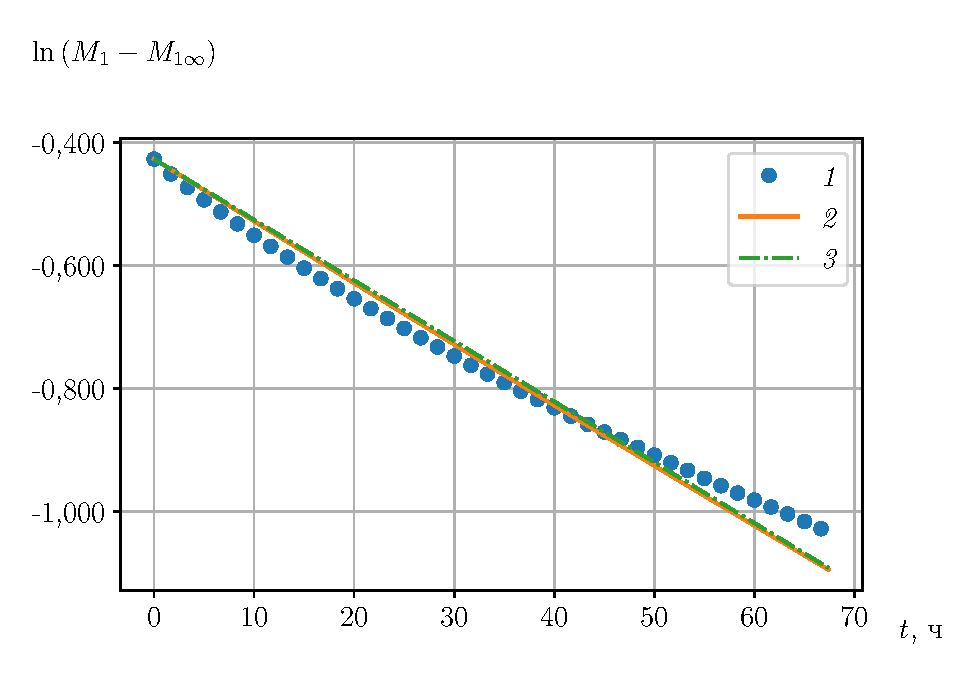
\includegraphics[width=17cm]{part_2/MS-V-1L_sorb_comp.pdf}\\
		\caption{Сорбционные зависимости, полученные различными способами для микросфер МС-В-1Л:
		\textit{1} -- экспериментальные данные;
		\textit{2} -- результаты расчета с учетом заданного распределения по размерам при $C_m=3,2\cdot 10^{-23}$~c;
		\textit{3} -- результаты расчета без учета неравномерности распределения по размерам при $C_m=3,1\cdot 10^{-23}$~c.}
		\label{pic:MS-V-1L_sorp_comp}
\end{figure}

В данном случае 
\begin{equation}
\label{eq:uneven_br_microsphere}
\beta(r) = \frac{3 C_m}{r d}\left(1+\displaystyle\frac{d}{r}\right) R_1 T,
\end{equation}
где $C_m$ -- неизвестная искомая константа. 

Подставляя (\ref{eq:uneven_br_microsphere}) в систему (\ref{eq:uneven_cont_model_qr}), получаем уравнение Фредгольма второго рода для определения $M_1(t)$ по заданным $q(r)$ и $C_m$. Варьируя $C_m$, можно подобрать некоторое значение, при котором достигается наилучшее соответствие экспериментальным данным (например, с помощью в метода наименьших квадратов). На рис. \ref{pic:MS-V-1L_sorp_comp}
приведены сорбционные зависимости, полученные экспериментально, а также рассчитанные по приведенной модели при $C_m=3,2\cdot 10^{-23}$~c и монодисперсной модели  (\ref{eq:permeation_even_laws_p}), в которой все микросферы считаются одинаковыми при $C_m = 3,1\cdot 10^{-23}$~c.

\textbf{Поглощение гелия ценосферами марки НМ-Р-5А - 0,16 мм (vv vac).}
Основные характеристики ценосферам НМ-Р-5А - 0,16 мм (vv vac) приведены в Приложении \ref{AppendixA}. Построим модель процесса поглощения на основе распределения $q(r)$, получаемого из известного распределения частиц по размерам рис. \ref{pic:HM-R-5A_distr}.

В отличие от толщины стенки микросферы, толщина стенки ценосферы $d$ зависит от размера частицы и в среднем пропорциональна радиусу полости $r$ с коэффициентом $\zeta=0,04$  \cite{Ver_Kurteeva}.

В данном случае с учётом сказанного выше получаем
\begin{equation}
\label{eq:uneven_br_HM-R-5A}
\beta(r) = 3 C_m R_1 T \frac{1+\zeta}{\zeta r^2} .
\end{equation}
Подставляя (\ref{eq:uneven_br_HM-R-5A}) в систему (\ref{eq:uneven_cont_model_qr}) получаем уравнение Фредгольма второго рода для определения $M_1(t)$ по заданным $q(r)$ и $C_m$. Варьируя $C_m$, можно подобрать некоторое значение, при котором достигается наилучшее соответствие экспериментальным данным. На рис. \ref{pic:HM-R-5A_sorb_comp} приведены сорбционные зависимости полученные экспериментально, а также рассчитанные по приведенной модели при $C_m=2,0\cdot 10^{-21}$~c и монодисперсной модели (\ref{eq:permeation_even_laws_p}) при $C_m = 1,0\cdot 10^{-21}$~с.

\begin{figure}[ht]
	\centering
	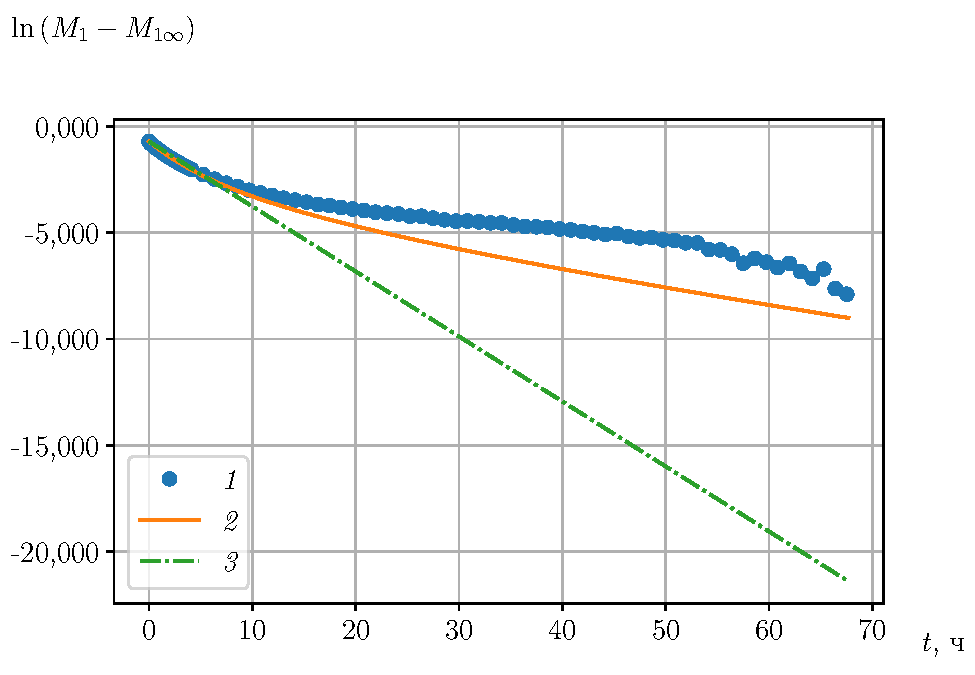
\includegraphics[width=0.9\textwidth]{part_2/HM-R-5A_sorb_comp.pdf}\\
	\caption{Сорбционные зависимости, полученные различными способами для ценосфер НМ-Р-5А - 0,16 мм (vv vac):
		\textit{1} -- экспериментальные данные;
		\textit{2} -- результаты расчета с учетом заданной неравномерности по размерам при $C_m=2,0\cdot 10^{-21}$~c;
		\textit{3} -- результаты расчета без учета неравномерности распределения по размерам при $C_m=1,0\cdot 10^{-21}$~c.
	}
	\label{pic:HM-R-5A_sorb_comp}
\end{figure}


%Установим предсказательную силу и проведём сравнение полученной математической модели (\ref{eq:uneven_cont_model_qr_dimensionless}) с простейшей из раздела \ref{section_2_1}.

%\podpunkt{Поглощение гелия микросферами марки <<МСВ1-Л>>} Параметры сорбента <<МСВ-1Л>>, а также сорбционные зависимости, полученные при различных начальных давлениях, приведены в \cite{Ver_Est_Perm}. Построим модель процесса поглощения на основе известного распределения $q(r)$ (рис. \ref{pic:microsphere},~а).
%
%В данном случае 
%\begin{equation}
%\label{br_microsphere}
%\beta(r) = \frac{3 C_m}{r d} R_1 T,
%\end{equation}
%где $C_m$ -- неизвестная искомая константа. 
%
%Подставляя (\ref{br_microsphere}) в систему (\ref{cont_model_qr_dimensionless}), получаем уравнение Фредгольма второго рода для определения $M_1(t)$ по заданным $q(r)$ и $C_m$. Варьируя $C_m$, можно подобрать некоторое значение, при котором достигается наилучшее соответствие экспериментальным данным (например, с помощью в метода наименьших квадратов). На рис. \ref{pic:microsphere},~б приведены сорбционные зависимости, полученные экспериментально, а также рассчитанные по приведенной модели при $C_m=3,2\cdot 10^{-23}$~c и модели из \cite{Ver_Est_Perm}, в которой все микросферы считаются одинаковыми при $C_m = 3,1\cdot 10^{-23}$~c.
%
%
%
%\podpunkt{Поглощение гелия ценосферами марки <<НМ-Р-5А - 0,16 мм (vv vac)>>} Построим модель процесса поглощения на основе известного распределения $q(r)$ (рис. \ref{pic:cenosphere}, а).
%
%В отличие от толщины стенки микросферы, толщина стенки ценосферы $d$ зависит от размера частицы и в среднем пропорциональна радиусу полости $r$ с коэффициентом $\gamma=0,04$  \cite{Ver_Kurteeva}.
%
%В данном случае с учетом сказанного выше получаем
%\begin{equation}
%\label{br_cenosphere}
%\beta(r) = \frac{3 C_m}{\gamma r^2} R_1 T.
%\end{equation}
%Подставляя (\ref{br_cenosphere}) в систему (\ref{cont_model_qr}) получаем уравнение Фредгольма второго рода для определения $M_1(t)$ по заданным $q(r)$ и $C_m$. Варьируя $C_m$, можно подобрать некоторое значение, при котором достигается наилучшее соответствие экспериментальным данным. На рис. \ref{pic:cenosphere}, б приведены сорбционные зависимости полученные экспериментально, а также рассчитанные по приведенной модели при $C_m=2,0\cdot 10^{-21}$~c и модели \cite{Ver_Est_Perm} при $C_m = 1,0\cdot 10^{-21}$~с.
%
%\punkt{Выводы.} В работе получена математическая модель поглощения гелия сорбентом, состоящим из полых сферических частиц в условиях дисперсионного распределения по приведенным коэффициентам проницаемости (включающего распределение как  по размерам, так и по коэффициентам проницаемости), представляющая собой уравнение Фредгольма второго рода для искомой кривой сорбции. 
%
%Показано, что по известному распределению микросфер по размеру при условии постоянства коэффициента проницаемости материала стенки можно восстановить сорбционную зависимость. В результате математического моделирования получены коэффициенты проницаемости для двух различных поглотителей. 
%
%Сравнение предлагаемой модели поглощения гелия микросферами  и модели из \cite{Ver_Est_Perm} показало, что
%в случае микросфер марки <<МСВ-1Л>> обе модели дают одинаковую сорбционную зависимость и рассчитанные коэффициенты проницаемости стенки частицы совпадают  c погрешностью, не превышающей 3~\%; 
%в случае ценосфер марки <<НМ-Р-5А - 0,16 мм (vv vac)>> учет зависимости толщины стенки от размера частиц в полученной модели позволяет получить более точную аппроксимацию. Рассчитанные коэффициенты проницаемости для сорбента на основе ценосфер по данной модели и модели из \cite{Ver_Est_Perm} отличаются в 2 раза.
%
%Авторы выражают благодарность С.~Н.~Верещагину за помощь при подготовке работы.

% Стиль списка литературы

%\renewcommand{\refname}{Литература}
%
%% ---------- весь блок важен ----------------
%\makeatletter
%\renewcommand{\@biblabel}[1]{#1.} % Заменяем библиографию с квадратных скобок на точку:
%\makeatother
%% ----------------------------------------------------
%
%\begin{thebibliography}{9}
%	
%	\bibitem{Kizil}
%	Кизильштейн Л. Я., Дубов И. В., Шпицглуз А. Л., Парада С. Г. Компоненты зол и шлаков ТЭС //  М.: Энергоатомиздат,
%	1995. 176~c.
%	
%	\bibitem{Ver_Est_Perm} 
%	Верещагин А. С., Зиновьев В. Н., Фомин  В. М. и др. Оценка коэффициента проницаемости стенок микросфер // Вестн. Новосиб. гос. ун-та. Сер.: Физика. 2010. Т. 5, \No~2. С. 8–16.
%	
%	\bibitem{Tsugawa}
%	Tsugawa  R. T., Moen I., Roberts P. E., Souers P. C. Permeation of helium and hydrogen from glass-microsphere laser
%	targets  // J. Appl. Phys. 1976. V. 47, N. 5. P. 1987–1993.
%	
%	\bibitem{ICCT_cenosphere_permeation}
%	Фоменко Е. В., Аншиц Н. Н., Панкова М. В. и др. Гелиевая проницаемость микросферических мембран на основе
%	муллитизированных ценосфер  // Докл. АН. 2010. Т. 435, \No~5. С. 640–642.
%	
%	\bibitem{ICCT_Ver_Cenosphere_Perm}
%	Черных Я. Ю., Верещагин С. Н. Исследование гелиевой проницаемости узкой фракции ценосфер энергетических зол // Журн. Сиб. федер. ун-та. Сер. Химия. 2011. Т. 4, \No~2. С. 137–147. 
%	
%	\bibitem{Argunova_Sorokin}
%	Аргунова Т. С., Сорокин Л. М., Певзнер Б. З. и др. Влияние дефектов кристаллической структуры на диффузию гелия в кварце // Физика твердого тела. 2003. Т. 45, \No~10. С. 1818–1824.
%	
%	\bibitem{Ver_Norm_Dist}
%	Верещагин А. C. Оценка влияния дисперсии нормального распределения радиуса полости на моделирование процесса поглощения гелия микросферами // Вестн. Новосиб. гос. ун-та. Сер.: Физика.  2011. Т. 6, \No~2. С. 24–27.
%	
%	\bibitem{Ver_Kurteeva}
%	Верещагин С. Н., Куртеева Л. И., Аншиц А. Г. Содержание ча-
%	стиц различного размера и плотности в концентратах ценосфер
%	летучих зол от сжигания углей Кузнецкого бассейна // Химия в
%	интересах устойчивого развития. 2008. Т. 16. С. 529–536.
%	
%\end{thebibliography}
%
%
%%\bibliographystyle{ugost2008}
%%\bibliography{./references}
%
%%\newcommand*{\rom}[1]{\expandafter\@slowromancap\romannumeral #1@}
%%\newcommand{\RNum}[1]{\uppercase\expandafter{\romannumeral #1\relax}}
%
%\begin{flushright} 
%	%\it
%	Поступила в редакцию 18/VI 2012 г.,\\
%	в окончательном варианте -- 4/X 2012 г.
%\end{flushright}
%
%
%
%
%\newpage
%\begin{figure}[H]
%	\centering
%	\includegraphics[width=17cm]{images/micro.pdf}\\
%	%\caption{cверху: плотность распределение радиуса полости микросфер МСВ-1Л, полученная методом лазерной дифракции;
%	%снизу: 
%	%1 -- экспериментальная сорбционная зависимость для микросфер МСВ-1Л;
%	%2 -- рассчитанная сорбционная зависимость с учетом заданного распределения по размерам для коэффициента проницаемости $C_m=3,2\cdot 10^{-23}$~c;
%	%3 -- рассчитанная сорбционная зависимость без учета неравномерности по размерам для коэффициента проницаемости $C_m=3,1\cdot 10^{-23}$~c. 
%	%}
%	\caption{}
%	\label{pic:microsphere}
%\end{figure}
%
%\newpage
%\begin{figure}[H]
%	\centering
%	\includegraphics[width=17cm]{images/ceno.pdf}\\
%	%\caption{Сверху: плотность распределение радиуса полости ценосфер НМ-Р-5А - 0,16 мм (vv vac), полученная эмпирическим путем;
%	%снизу: 
%	%1 -- экспериментальная сорбционная зависимость для ценосфер НМ-Р-5А - 0,16 мм (vv vac); 
%	%2 -- рассчитанная сорбционная зависимость с учетом заданного распределения по размерам для коэффициента проницаемости $C_m=2,0\cdot 10^{-21}$~c;
%	%3 -- рассчитанная сорбционная зависимость без учета неравномерности распределения по размерам для коэффициента проницаемости $C_m=1,0\cdot 10^{-21}$~c.  $M_{1\infty}$ -- равновесное значение массы гелия вне частиц, одинаковое для всех приведенных экспериментов.}
%	\caption{}
%	\label{pic:cenosphere}
%\end{figure}
%
%
%\newpage
%Рис. 1. Кривые сорбции для микросфер <<МСВ-1Л>>:
%
%а -- плотность распределения радиуса полости микросфер, полученная методом лазерной дифракции;
%б -- сорбционные зависимости, полученные различными способами 
%(\textit{1} -- экспериментальные данные,
%\textit{2} -- результаты расчета с учетом заданного распределения по размерам при $C_m=3,2\cdot 10^{-23}$~c,
%\textit{3} -- результаты расчета без учета неравномерности распределения по размерам при $C_m=3,1\cdot 10^{-23}$~c).
%
%
%\newpage
%Рис. 2. Кривые сорбции для ценосфер <<НМ-Р-5А - 0,16 мм (vv vac)>>:
%
%a -- плотность распределения радиуса полости ценосфер, полученная эмпирически;
%б -- сорбционные зависимости, полученные различными способами 
%(\textit{1} -- экспериментальные данные,
%\textit{2} -- результаты расчета с учетом заданной неравномерности по размерам при $C_m=2,0\cdot 10^{-21}$~c,
%\textit{3} -- результаты расчета без учета неравномерности распределения по размерам при $C_m=1,0\cdot 10^{-21}$~c).







\section{Моделирование поглощения гелия композитным сорбентом на основе микросфер}
\label{section_2_4}

